\lettrine{I}{n} this section the paper is going to solve three of the four main problems:

\begin{itemize}
    \item Policies latency and consistency
    \item Hacking of the Roles with Message Tempering
    \item Hacking of the Roles with Messages using Policies is no longer Allowed.
\end{itemize}

\subsection{Policies latency and consistency}
\label{sec:policies-latency-consistency}

The evaluation of a policy can be accomplished using an evaluation function, denoted as $f_{eval}$.

This function takes as input an identity, a resource, and an action. 
Subsequently, it evaluates whether the specified action can be performed on the given resource.

\begin{boxF}
    \begin{definition}[UUR Matching Algorithm - $f_{uurmatch}$]
        The function $f_{uurmatch}$ is designed to take two Uniform Resource Identifiers (UURs) as input and returns a Boolean value.
        
        Specifically, it returns True if the first $UUR$, denoted as $uur1$, is matched within the second $UUR$, denoted as $uur2$. 
        
        An UUR is considered to be matched if the two are identical or if $uur2$ has wildcards that permit the match of $uur1$.
    \end{definition}
\end{boxF}

\begin{boxF}
    \begin{definition}[Policy Evaluation Algorithm - $f_{eval}$]
        Input:
        \begin{itemize}
            \item iid: identifier of the identity to be evaluated
            \item iurr: resource to be evaluated
            \item iaction: action to be evaluated
            \item P: set of the policies
            \item PI: set of the policies associated to the identities
        \end{itemize}
        Output: true if the action cen be performed on the input resource, false otherwise.

        BEGIN:
            
        \hspace{2pt} $DP = \sigma_{IdentityId=iid, Effect='deny'}(PI \bowtie P)$
        
        \hspace{2pt} $DPA = \pi_{UUA}(\sigma_{f_{uurmatch}(iurr, UUR)}(DP)$)

        \hspace{2pt} $\forall action_{DP} \in DPA,$
            
        \hspace{10pt} if $action_{DP} = iaction$ return false
        \vspace{10pt}
        
        \hspace{2pt} $AP = \sigma_{IdentityId=iid, Effect='allow'}(PI \bowtie P)$

        \hspace{2pt} $APA = \pi_{UUA}(\sigma_{f_{uurmatch}(iurr, UUR)}(AP)$)

        \hspace{2pt} $\forall action_{AP} \in APA,$
            
        \hspace{10pt} if $action_{AP} = iaction$ return true
        \vspace{10pt}

        \hspace{2pt} return false
        \label{definition:policy-evaluation}
    \end{definition}
\end{boxF}

A software solution necessitates invoking the $f_{eval}$ function for each required policy enforcement. 
In the scenario where the solution must evaluate whether an action can be performed on a resource $n$ times, the function has a time complexity $O(n)$.

\vspace{15pt}

This level of complexity would be acceptable only under the condition that the execution time for each function call is very short, in the range of a few milliseconds. 
However, each evaluation point would demand a call to a remote server to evaluate the policy, introducing significant latency to the overall solution and rendering the system unavailable in the event of network partitioning.


\vspace{15pt}

The time-consuming operations in the implementation of the Policy Evaluation Algorithm ~\ref{definition:policy-evaluation} are those executing queries, such as selections and projections. 
The only way to reduce this execution time and the risk of network partitioning is to minimize the number of remote queries and execute them locally. 

\vspace{15pt}

This can be achieved by synchronizing the policies into the node and loading all of them into memory. 
While this approach would resolve the latency and network partitioning issues, it introduces the trade-off of eventually consistent data, and the node might experience periods where policies are out of synchronization as shown in Figure \ref{fig:policies-enf-latency-and-consistency}.

\begin{figure}[h]
    \centering
    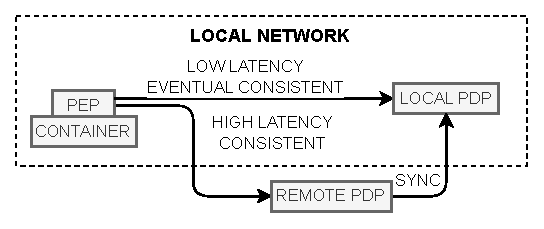
\includegraphics[width=\linewidth]{policy-based-apporach/policies-enf-latency-and-consistency.pdf}
    \caption{Latency and Consistency for Policies Enforcement}
    \label{fig:policies-enf-latency-and-consistency}
\end{figure}

\subsection{Hacking of the Roles with Messages}
\label{sec:hacking-role-messages-solution}

A software solution implementing asynchronous operations backed by messages would need to assess the permissions of the identity for the requested action on a resource. 
Upon successful evaluation, it would publish a message. On the receiving end, a consumer would read the message and execute the action.

\vspace{15pt}

Let's consider a scenario where the identity $email-2$ has been granted permissions by the policies $p1, p3, p4, p5$ and the identity requests to create an order, resulting in the publication of a message with the request to create an order for the identity $email-2$ which is granted by the policy $p4$.

\vspace{15pt}

The consumer node would need to perform the operation on behalf of the identity; therefore, the functional account used to execute the consumer would require the permission $p4$. 

\vspace{15pt}

While it's possible to assign the permissions granted by the policies $p1, p3, p4, p5$ to the functional account, doing so would expose the system to multiple security risks:
\begin{itemize}
    \item \textbf{Separation of Concern}: A consumer implementing OMS-System features should not implement Banking-System features.
    \item \textbf{Least Privilege Principle}: The consumer should adhere to the principle of least privilege, which is a concept that restricts a user's access rights to only what is strictly necessary.
\end{itemize}

\vspace{15pt}

It is correct to consider assigning only the permissions granted by the $p4$ policy to the functional account. 
However, a challenge arises as this consumer needs to handle all types of requests for the OMS-System.

As a result, granting the service account all the permissions from all OMS-System policies would be necessary. 
However, this would expose the system to security risks and would not adhere to the principle of least privilege.

\vspace{15pt}

Let's define $M1$ as the set of policies required to execute the action in the message $m_1$, denoted as $M1 = \{p_i, p_j\}$. Similarly, let's define $M2$ as the set of policies required to execute the action in the message $m_2$, denoted as $M2 = \{p_m, p_n\}$. 
The security risks would be defined as following:
\begin{itemize}
    \item When executing $m_1$, security risks would be introduced by the policies that are not required to execute the operation, specifically $M2 - (M1 \cap M2)$
    \item When executing $m_2$, security risks would be introduced by the policies that are not required to execute the operation, specifically $M1 - (M1 \cap M2)$
\end{itemize}

\vspace{15pt}

This leads to the concept of a runtime policy evaluation context. This implies that when serving a request, the service account should be running in a runtime policy evaluation context that includes only the strictly required policies. 
In the previous usage example, when processing the message $m_1$, the runtime policy evaluation context should include the policies in $M1$, while when processing $m_2$, the context should include the policies in $M2$.

This can be achieved by requiring the system to specify, in each message, the requesting identity and the role required to execute the message. On the other hand, the consumer would need to be granted permissions to impersonate the identity specified in the message by elevating its own identity to the specified role.

\begin{figure}[h]
    \centering
    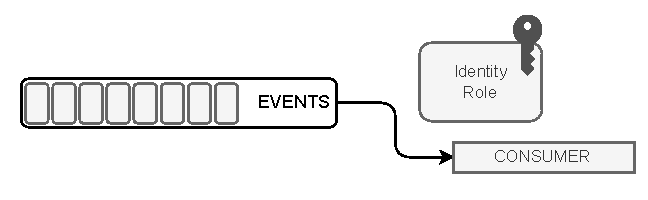
\includegraphics[width=\linewidth]{policy-based-apporach/hacking-role-message-signature.pdf}
    \caption{Message processing}
    \label{fig:hacking-role-message-signature}
\end{figure}

To prevent falling victim to a message tampering attack, the ACS solution requires signing messages and mandates that consumers verify the validity of each message.

\begin{boxF}
    \begin{definition}[Message processing by Role - $f_{process}$]
        Input:
        \begin{itemize}
            \item msg: message to be processed
        \end{itemize}

        BEGIN:

            \hspace{2pt} // Validate the signature of the message

            \hspace{2pt} $f_{validate}(msg)$

            \hspace{2pt} // Elevate the identity to be executed as the role in the message

            \hspace{2pt} $f_{elevate-role}(msg)$

            \hspace{2pt} // Process the message
        \label{definition:message-processing}
    \end{definition}
\end{boxF}

\vspace{15pt}

\subsection{Hacking of the Roles with Messages using Policies is no longer Allowed}
\label{sec:hacking-republish-message-solution}

A software solution would need to evaluate the actions on resources for each identity request and subsequently execute the action on the system. 
However, during the interval between the evaluation of the action and its execution, the permissions associated with the identity might have changed.
This becomes more pronounced in distributed systems utilizing asynchronous operations supported by messages.

The Message Processing by Role Algorithm ~\ref{definition:message-processing} enables the handling of this type of issue as well. 
By requiring a consumer to elevate its identity to a specific role, it ensures that at the time of execution, the latest policies are applied to the role. 
Therefore, if there are changes since the point in time when the identity made the request, these changes would be reflected in the execution of the asynchronous operation.
